\documentclass[12pt, a4paper]{article}

\usepackage[english]{babel}

\usepackage{cite}
\usepackage{hyperref} % \autoref

\usepackage[pdftex]{graphicx}
\graphicspath{{pic/}}
\usepackage{tikz}

\usepackage{amsmath,amsfonts,amssymb,amsthm,amscd,amsxtra}
\usepackage{mathtools}

\theoremstyle{plain}
\newtheorem{theorem}{Theorem}


\newcommand{\mcL}{\mathcal{L}} % L2 space
\newcommand{\mcO}{\mathcal{O}} % Big O
\newcommand{\bbC}{\mathbb{C}} % complex plane
\newcommand{\bbD}{\mathbb{D}} % complex unit disk
\newcommand{\bbR}{\mathbb{R}}
\newcommand{\bbT}{\mathbb{T}} % complex unit circle
\newcommand{\bbH}{\mathbb{H}} % complex upper half plane

% imaginary unit
\newcommand{\iu}{{i\mkern1mu}}

% \renewcommand{\Re}{\operatorname{Re}}
% \renewcommand{\Im}{\operatorname{Im}}

\newcommand{\eexp}[1]{e^{#1}}

\renewcommand{\Re}{\operatorname{Re}}
\renewcommand{\Im}{\operatorname{Im}}
\DeclarePairedDelimiter\abs{\lvert}{\rvert}%
\DeclarePairedDelimiter\norm{\lVert}{\rVert}%

\DeclareMathOperator\asin{asin}
\DeclareMathOperator\atanh{atanh}

\begin{document}

\section{Introduction}
TODO ?????

\section{Definitions}
\begin{itemize}
\item $\bbC$: complex plane, $\bbC = \{ x + \iu y \mid x, y \in \bbR \}$ 
\item $\bbH$: upper complex half-plane, $\bbH = \{ x + \iu y \mid y > 0, x, y \in \bbR \}$
\item $\bbD$: unit disk, $\bbD = \{ z \mid \abs{z} < 1 \}$
\item $\bbT$: unit circle, $\bbT = \partial \bbD =  \{z \mid \abs{z} = 1 \}$
\item $z$ denotes a complex argument on upper complex half-plane $\bbH$
\item $\zeta$ denotes a complex argument on unit disk $\bbD$
\end{itemize}

\section{Schrodinger's equation}
In this paper we are only interested in the mathematical scattering problem and not actual energies, so we define Plank's constant as $1$ and use stationary Schrodinger's equation: $H \Psi = E \Psi$. We are going to be interested in scattering state solutions for this equation.

\section{S-matrix}\label{sec:smatrix}
Consider a localized one dimensional potential barrier or resonator. From the left and right we subject in to beams of quantum particles with the wavevector $k$ (which will be a scalar in 1D case). Outside the potential barrier the particles behave as plane waves:

\begin{equation}\label{eq:wlwl}
\begin{aligned}
   \psi_L(x) &= A \eexp{\iu k x} + B \eexp{-\iu k x}
\\ \psi_R(x) &= C \eexp{\iu k x} + D \eexp{-\iu k x}
\end{aligned}
\end{equation}

S-matrix, or scattering matrix relates the final and initial states of the system:
\begin{equation}\label{eq:smatrix}
\begin{pmatrix} B \\ C \end{pmatrix} = S \begin{pmatrix} A \\ D \end{pmatrix}
\end{equation}
, and defines scattering properties of a potential barriers.

\section{Cayley transform}

Cayley transform maps $\bbH$ to $\bbD$:
\begin{equation}\label{eq:cayley}
W(z) = \frac{z - \iu}{z + \iu}
\end{equation}
, inverse Cayley transform maps $\bbD$ to $\bbH$:
\begin{equation}\label{eq:cayley_inverse}
w(\zeta) = \iu \frac{1 + \zeta}{1 - \zeta}
\end{equation}

One notable property of the Cayley transform is that it injectively maps $\bbR$ into unit circle $\bbT$.

Another important property we are going to use is that Cayley transform preserves circles. In particular, a circle with radius $r < 1$ centered in zero, under inverse Cayley transform maps into a circle with center $\iu C(r)$ and radius $R(r)$, where:

\begin{equation}\label{eq:c_and_r}
\begin{aligned}
   C(r) &= \Im \frac{w(r) + w(-r)}{2} = \frac{1 + r^2}{1 - r^2}
\\ R(r) &= \Im \frac{w(r) - w(-r)}{2} = \frac{2 r}{1 - r^2}
\end{aligned}
\end{equation}

From these formulas it's easy to see that if we limit $r$ to $1$, $R(r)$ goes to infinity and $C(r)$ converges to $R(r)$, which intuinively makes sense since a complex unit circle maps to a real axis.

Also, we'll note two useful facts:
\begin{itemize}
\item $C(r) - R(r) > 0$
\item $C(r) - R(r) = \frac{1 - r}{1 + r} < \frac{1}{R(r)} = \frac{1 - r^2}{2 r}$, which means that $C - R$ is $\mcO(\frac{1}{R})$
\end{itemize}

% TODO: $C(r) + R(r) = \Im w(r) = \frac{1 + r}{1 - r}$, $C(r) - R(r) = \Im w(-r) = \frac{1 - r}{1 + r}$

\section{Convergence criterion}
There is a connection between the S-matrix and the completeness of the resonant states for a scattering problem:

TODO something about dissipating operator

\begin{theorem}[{\cite[p. 95]{nikol2012treatise}}, {\cite[p. 99]{nikol2012treatise}}]
The following statements are equivalent:
\begin{itemize}
\item the dissipating operator $Z$ is complete
\item
\begin{equation}\label{eq:blaschke}
\lim\limits_{r = 1} \int\limits_{\bbT} \log \abs{\det S(r \zeta)} d m(\zeta) = 0
\end{equation}
\end{itemize}
\end{theorem}

Next, we will use the criterion \ref{eq:blaschke} to analyse the completeness of the system of resonant states. In the space of the unit disk it looks like:
\begin{equation}\label{eq:crit_cayley}
\lim\limits_{r = 1} \int\limits_{\abs{\zeta} = r} \log \abs{\det S(\zeta)} d \zeta = 0
\end{equation}

Since S-matrix is naturally defined on the complex plance, it makes sense to use the upper complex plane for the analysis of completeness. We change the variable in (\ref{eq:crit_cayley}), applying Cayley transform to the integral, which results in:

\begin{equation}\label{eq:crit}
\lim\limits_{r \to 1} \int\limits_{C_r} \ln \abs{\det S(k)} \frac{2 \iu}{(k + i)^2} dk = 0
\end{equation}
, where $C_r$ is an image of $\abs{\zeta} = r$ under the inverse Cayley transform. It can be parameterised as $C_r = \{R(r) \eexp{\iu t} + \iu C(r) \mid t \in [0, 2 \pi)\}$ (see \ref{eq:c_and_r}). For brewity, define:

\[
s(k) = \abs{\det S(k)}
\]
, and after throwing away constants which are irrelevant for convergence, we get the final form of the criterion, which we are going to use afterwards:

\begin{equation}\label{eq:critp}
\lim\limits_{r \to 1} \int\limits_{0}^{2 \pi} \ln s(R(r) \eexp{\iu t} + \iu C(r)) \frac{R}{(R(r) \eexp{\iu t} + \iu C(r) + i)^2} dt = 0
\end{equation}


\section{The model}
% TODO http://tex.stackexchange.com/a/155317/5966 ?
\begin{figure}
\centering
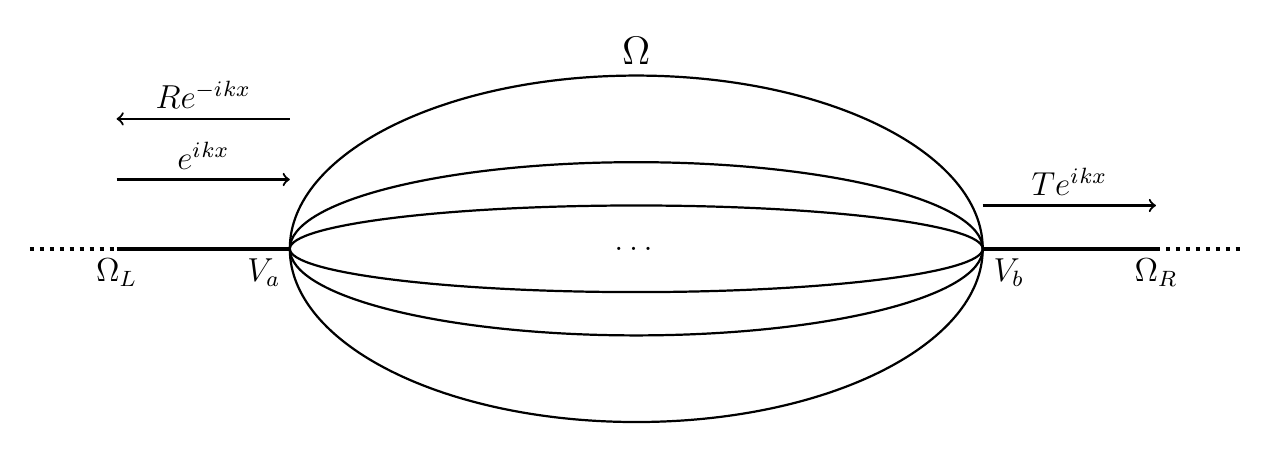
\begin{tikzpicture}[scale=1.1] % TODO SCALE!!!
\newcommand{\Wglen}{6.0}; % waveguide length
\newcommand{\Warrlen}{2.0}; % wave arrow length
\newcommand{\Reslen}{4.0}; % resonator length

\coordinate (LLL) at (-\Wglen - 1, 0);
\coordinate (RRR) at ( \Wglen + 1, 0);
\coordinate (LL)  at (-\Wglen, 0);
\coordinate (RR)  at ( \Wglen, 0);
\coordinate (L)   at (-\Reslen, 0);
\coordinate (R)   at ( \Reslen, 0);
%

\coordinate (U) at (0, 3); % upper point of resonator

% waveguide
\draw[ultra thick, dotted] (LLL) -- (LL);
\draw[ultra thick] (LL)--(L);
\draw[ultra thick] (R)--(RR);
\draw[ultra thick, dotted] (RR) -- (RRR);
%

\draw[<-, thick] (-\Wglen, 1.5) -- (-\Wglen + \Warrlen, 1.5) node [midway, above] {\large $R e^{-\iu k x}$};
\draw[->, thick] (-\Wglen, 0.8) -- (-\Wglen + \Warrlen, 0.8) node [midway, above] {\large $e^{\iu k x}$};
\draw[->, thick] (\Wglen - \Warrlen, 0.5) -- (\Wglen, 0.5)   node [midway, above] {\large $T e^{\iu k x}$};

\draw (LL) node [below] {\large $\Omega_L$};
\draw (RR) node [below] {\large $\Omega_R$};

\draw[ultra thick] (0, 2) node [above] {\Large $\Omega$};

% \draw[ultra thick] node [below] {$V$} (0, 2) circle[radius=2] 
\draw[thick] (4,0)  arc[x radius = 4cm, y radius = 2cm, start angle= 0, end angle=180];
\draw[thick] (4,0)  arc[x radius = 4cm, y radius = 1cm, start angle= 0, end angle=180];
\draw[thick] (4,0)  arc[x radius = 4cm, y radius = 0.5cm, start angle= 0, end angle=180];
\draw[thick] (-4,0)  arc[x radius = 4cm, y radius = 2cm, start angle= 180, end angle=360];
\draw[thick] (-4,0)  arc[x radius = 4cm, y radius = 1cm, start angle= 180, end angle=360];
\draw[thick] (-4,0)  arc[x radius = 4cm, y radius = 0.5cm, start angle= 180, end angle=360];

\draw (-\Reslen - 0.3, 0) node [below] {\large $V_a$};
\draw ( \Reslen + 0.3, 0) node [below] {\large $V_b$};
\draw (0, 0) node {\large $\dots$};
\end{tikzpicture}
\caption{Quantum graph $\Gamma$, consisting of semi infinite edges $\Omega_L, \Omega_R$ and a resonator $\Omega$, consisting of $W$ identical edges of length 1.}
\label{fig:res_bundle}
\end{figure}

Let's investigate the model on \autoref{fig:res_bundle}. Schrodinger's operator is defined on edges of the graph as  $-\frac{d^2 \psi}{dx^2}$. At the vertices $V_a$ and $V_b$ we require the wavefunction and its derivatives to be continuous:

\begin{equation}\label{eq:bundle_system}
\begin{aligned}
   \forall i: \psi_i(0) &= \psi_L(0)
\\ \forall i: \psi_i(1) &= \psi_R(0)
\\ \psi'_L(0) - \sum\limits_{i = 1}^W \psi'_i(0) &= 0
\\ -\psi'_R(0) + \sum\limits_{i = 1}^W \psi'_i(1) &= 0
\end{aligned}
\end{equation}

\subsection{Calculation of $S$ matrix}
After solving \ref{eq:bundle_system} in conjunction with \ref{eq:wlwl}, we get:
\begin{equation*}
\det S(k) = \frac{2 i \, W \cos\left(k\right) - {\left(W^{2} + 1\right)} \sin\left(k\right)}{2 i \, W \cos\left(k\right) + {\left(W^{2} + 1\right)} \sin\left(k\right)}
\end{equation*}


\begin{equation}\label{eq:bundle_s}
s(k) = \abs{\det S(k)} = \abs{\frac{2 i \, W \cos\left(k\right) - {\left(W^{2} + 1\right)} \sin\left(k\right)}{2 i \, W \cos\left(k\right) + {\left(W^{2} + 1\right)} \sin\left(k\right)}}
\end{equation}

TODO: define contour

Let's fix $r$, and further, for the sake of readability, let's define $C = C(r)$ and $R = R(r)$. For each $r$, we estimate the integral and show that the sequence of estimates converges to zero.

Let's use Cauchy-Schwarz's inequality:
\[
\big| \langle u,v \rangle \big| \leq \left\|u\right\| \left\|v\right\|
\]
, to be precise, it's $\mcL^2[a, b]$ version:
\[
\abs{
\int\limits_{t=a}^{b} f(t) g^*(t) dt
}
\le
\sqrt{\int\limits_{t=a}^b \abs{f(t)}^2 dt }
\sqrt{\int\limits_{t=a}^b \abs{g(t)}^2 dt }
\]
% 
To use inequality, we are going to represent the integrand in (\ref{eq:critp}) as $f(t) g^*(t)$ as follows:
\begin{equation}\label{eq:split}
\begin{aligned}
a      &= 0 \\
b      &= 2 \pi \\
f(t)   &= \ln s(R \eexp{\iu t} + \iu C) \frac{\sqrt{R}}{R \eexp{\iu t} + \iu C + i} \\
g^*(t) &= \frac{\sqrt{R}}{R \eexp{\iu t} + \iu C + i}
\end{aligned}
\end{equation}
Next, we will show that $\norm{g}$ (that is, $\sqrt{\int \abs{g(t)}^2}$) is bounded by a constant which does not depend on $r$, and $\norm{f}$ goes to $0$ as $r$ goes to $1$, hence (\ref{eq:critp}) converges.

\subsection{Estimating $\norm{g}$}

First, we evaluate the integrand:
\begin{align*}
\abs{g(t)}^2 = \abs{g^*(t)}^2
&=   \frac{\sqrt{R}^2}{\abs{R \cos t + \iu R \sin t + \iu C + i}^2} \\
&=   \frac{R}{R^2 \cos^2 t + (R \sin t + C + 1)^2} \\
&= \frac{R}{R^2 \cos^2 t + R^2 \sin^2 t + (C + 1)^2  + 2 R (C + 1) \sin t} \\
&=   \frac{1}{R + \frac{(C + 1)^2}{R} + 2 (C + 1) \sin t} \\ 
\end{align*}

We have to integrate this function on interval $[0, 2 \pi]$. Integral of such type is well-known: % REFTODO
\[
\int\limits_{0}^{2 \pi} \frac{dx}{a + b \sin x} = \frac{2 \pi}{\sqrt{a^2 - b^2}}
\]
, when $a > b$. In our case, $a = R + \frac{(C + 1)^2}{R}$, $b = 2 (C + 1)$).

First, we check that $a > b$:
\begin{align*}
   R + \frac{(C + 1)^2}{R} - 2 (C + 1)
   &= \frac{R^2 + C^2 + 2C + 1 - 2 RC - 2 R}{R}
\\ &= \frac{(C - R)^2 + 2(C - R) + 1}{R}
\\ &= \frac{(C - R + 1)^2 }{R}
\\ &> 0 && \text{,strictly greater since $C > R$} 
\end{align*}

Next, we compute en estimate for $\sqrt{a^2 - b^2}$:
\begin{align*}
a^2 - b^2
& =  (R + \frac{(C + 1)^2}{R})^2 - (2 (C + 1))^2\\
& =  R^2 + \frac{(C+1)^4}{R^2} + 2 (C+1)^2 - 4 (C + 1)^2 \\
& =  \left( \frac{(C + 1)^2}{R} - R \right)^2 \\
& =  \left( \frac{(C + 1)^2 - R^2}{R}\right)^2 \\
& =  \left( \frac{(C + 1 - R) (C + 1 + R)}{R}\right)^2 && \text{,since $C > R > 0$} \\
&\ge \left( \frac{(1) (R + R)}{R}\right)^2  \\
&\ge 4
\end{align*}

Finally, since $\frac{2 \pi}{\sqrt{a^2 - b^2}} \le \frac{2 \pi}{2} = \pi$, and we just proved that $\norm{g}$ is bounded by a constant. 


\subsection{Estimating $\norm{f}$}
Function $s(k)$ (\ref{eq:bundle_s}) is too complex for direct proof of the convergence.

We proceed as follows:

\begin{itemize}
\item Since $s(k)$ is an absolute value of the determinant of the $S$ matrix, in the upper complex plane $0 \le s(k) \le 1$ holds. From here, we immediately know that the integral is bounded from above since $ln^2 1 = 0$.
\item We replace $s(k)$ with a lower bound $l(k)$ such that: $0 \le l(k) \le s(k) \le 1$.
\item By appling logarithm to the expression above, we get $\ln l(k) \le \ln s(k) \le 0$, and therefore, $\ln^2 s(k) \le \ln^2 l(k)$.
\item Now, if we prove convergence for $l(k)$, this immediately proves the convergence of the original integral.
\end{itemize}

We are going to use this fact in our proof and do such function changes under the integral sign, replacing complicated function with simpler (in particular, piecewise linear) lower bounds, and then using well known facts to estimate the integral.

\subsubsection{Simplifying $s(k)$}
We build a simple estimate for $s(k)$ over the upper complex plane. This function will be independent of the complex part of its argument which will make the analysis way easier.

\begin{enumerate}
\item
  It is easy to spot that if we fix the complex part of the argument, $s(k)$ is periodic with respect to the real part of its argument.
\item 
  Function $s(k)$ has countably infinite set of zeros, and each of them has $\Im k = \atanh \frac{2 W}{W^2 + 1}$. For brewity, we define:

  \begin{equation*}
  \begin{aligned}
     V &= \frac{2 W}{W^2 + 1}
  \\ Z &= \atanh V
  \end{aligned}
  \end{equation*}
\item
  Notice that for each $x$, $s(x + \iu y) \le s(\iu y)$.
  % \mtodo{How to prove? We could probably take a look at numerator and denominator in separate?} 
\end{enumerate}

Given these facts, we can build a simple lower bound for $s(x + \iu y)$:
\begin{align*}
l(x + \iu y)
   &= \abs{\frac{(W^2 + 1) \sinh y - 2 W \cosh y}{(W^2 + 1) \sinh y + 2 W \cosh y}}
\\ &= \abs{\frac{\tanh y - V}{\tanh y + V}} && \text{(since $\cosh y > 0$)}
\end{align*}

It's pretty clear that $l(k)$ has a continuum of zeros over the line $\Im k = Z$, which implies that $\ln l(k)$ has continuum number of singularities over this line. Intuitively, it shouldn't spoil the convergence of integral since the contour of integration cound intersect the singularities of the original function anyway. And indeed, we will give a rigorous argument that we still can prove convergence in this case. Since the function is independent from the real part of the argument now, for brewity, we will omit it and defince $l(y) = l(\iu y)$.
% \mtodo{Plot?}

Now, we will simplify the integral using the bound we just constructed:
\begin{align*}
       \int\limits_{t=0}^{2 \pi} \abs{f(t)}^2 dt
   = & \int\limits_{t = 0}^{2 \pi} \ln^2 l(R \eexp{\iu t} + \iu C) \frac{R}{\norm{R \eexp{\iu t} + \iu C + i}^2} dt
\\ = & \int\limits_{t = 0}^{2 \pi} \ln^2 l(R \sin t + C) \frac{R}{R^2 \cos^2 t + (R \sin t + C + 1)^2} dt
\end{align*}

First, notice that:

\begin{equation*}
\begin{aligned}
   \sin(-\pi/2 + t)   &= \sin(-\pi/2 - t) = - \cos t
\\ \cos^2(-\pi/2 + t) &= \cos^2(-\pi/2 = t) = \sin^2 t
\end{aligned}
\end{equation*}
, that is, the integrand is symmetric with respect to $y$ and for proving convergence it is enough to prove convergence on the (half circle) contour defined by $-\pi/2 \le t \le \pi/2$.

Next, we do a variable change:
\begin{equation*}
\begin{aligned}
   y         &= R \sin t + C
\\ t         &= \asin \frac{y - C}{R}
\\ dt        &= \frac{1}{\sqrt{R^2 - (C - y)^2}} dy
\\ \cos t    &= \frac{\sqrt{R^2 - (C - y)^2}}{R}
\\ y(-\pi/2) &= C - R 
\\ y(\pi/2)  &= C + R 
\end{aligned}
\end{equation*}
, and after substitution:
\begin{equation}\label{eq:int_f}
\resizebox{0.9\hsize}{!}{$
\begin{aligned}
    & \int\limits_{y = C - R}^{C + R} \ln^2 f(y) \frac{R}{R^2 \cos^2 t + (R \sin t + C + 1)^2} dy \\
=   & \int\limits_{y = C - R}^{C + R} \ln^2 f(y) \frac{R}{R^2 - (C - y)^2 + (y + 1)^2} \frac{1}{\sqrt{R^2 - (C - y)^2}} dy\\
=   & \int\limits_{y = C - R}^{C + R} \ln^2 f(y) \frac{R}{R^2 - C^2 + 2 (C + 1) y + 1} \frac{1}{\sqrt{R + C - y}} \frac{1}{\sqrt{R - C + y}}  dy\\
\end{aligned}
$}
\end{equation}

On the integration path we cross singularities at $y = C - R$, $y = Z$, $y = C + R$, and the integrand is still too complex for direct estimation. Let's split the integration path in multiple segments and estimate them independently.

\subsubsection{Case 1: $C - R \le y \le Z$}
A crucial property of $s(k)$ is its convergence to 1 as $\Im k$ goes to 0 (which is because $s$ is the determinant of S-matrix), since then $\ln s(k)$ goes to zero, which is necessary to compensate the singularity of $\frac{1}{R - C + y}$ at $y = C - R$. 
This means that to prove convergence using lower bound for $s(k)$, we have to require that $s(k)$ also converges to $1$ as $\Im k$ goes to $0$.

% TODO plot?
Since $l$ is convex when $0 \le y \le Z$, we can estimate it from below using its first derivative at $0$. However, this is not enough, since it will this will violate the property of the estimate being positive (it is under the logarithm sign), so we have to be more careful and approximate the function at $Z$ with its first derivative as well, and then glue them together at some point $Z_0$:
\begin{align*}
f(y)
& = 
\begin{cases}
l'(0) y + 1   &, 0 \le y < Z_0  \\
l'(Z) (y - Z) &, Z_0 \le y < Z \\
\end{cases}
\\
& =
\begin{cases}
\frac{-2}{V} y + 1   &, 0 \le y < Z_0  \\
\frac{1}{2 V}(V^2 - 1) (y - Z) &, Z_0 \le y < Z \\
\end{cases}
\end{align*}

Note that lower bound does not have to be a continuous function, so we can pick any number in $[C - R, Z)$ as $Z_0$. For the ease of calculations, let's take $Z_0 = \frac{V}{4}$.  % \mtodo{plot?}

Next we compute upper bounds for the integral \ref{eq:int_f} on $[C - R, \frac{V}{4})$ and $[\frac{V}{4}, Z)$ separately.

\subsubsection{$C - R \le y < \frac{V}{4}$}

Note that for $C - R \le y \le \frac{V}{4}$:
\begin{align*}
       & \int \ln^2 l(y) \frac{R}{R^2 - C^2 + 2 (C + 1) y + 1} \frac{1}{\sqrt{R + C - y}} \frac{1}{\sqrt{R - C + y}}
\\ \le & \int \ln^2 (1 - \frac{2}{V} y) \frac{R}{R^2 - C^2 + 2 (C + 1) y + 1} \frac{1}{\sqrt{R + C - Z}} \frac{1}{\sqrt{R - C + y}}
\end{align*}

Now, we use a well known inequality which holds for $x > -1$: % REFTODO
\[
\frac{x}{1 + x} \le \ln (1 + x)
\]
, where in our case $x = -\frac{2}{V} y$. Since the expression under logarithm is less than 1, we get $\ln^2 (1 + x) \le \frac{x^2}{(1 + x)^2}$:
\begin{align*}
       & \dots 
\\ \le & \int \frac{\frac{4}{V^2}y^2}{(1 - \frac{2}{V}y)^2}  \frac{R}{R^2 - C^2 + 2 (C + 1) y + 1} \frac{1}{\sqrt{R + C - Z}} \frac{1}{\sqrt{R - C + y}}
\\ \le & \int \frac{\frac{4}{V^2}y^2}{(1 - \frac{2}{V} \frac{V}{4})^2}  \frac{R}{R^2 - C^2 + 2 (C + 1) y + 1} \frac{1}{\sqrt{R + C - Z}} \frac{1}{\sqrt{R - C + y}}
\\ =   & \frac{\frac{4}{V^2}}{(1 - \frac{2}{V} \frac{V}{4})^2} \frac{R}{\sqrt{R + C - Z}}  \int \frac{y^2}{R^2 - C^2 + 2 (C + 1) y + 1}  \frac{1}{\sqrt{R - C + y}}
\end{align*}

It's clear that the multiplier before the integral has order $\mcO(\sqrt{R})$ (we can ignore the terms dependent on $V$ only since $V$ is a constant independent of $r$).

The first part of the integrand has the form $\frac{y^2}{a + b y}$, where $a = R^2 - C^2 + 1, b = 2 (C + 1)$; when $R$ and $C$ are big enough, $a > 0$ and $b > 0$. That means $\frac{y^2}{a + b y}$ will be nonnegative when $y > 0$, and non decreasing, since:
\[
  \left(\frac{y^2}{a + b y}\right)'
= \frac{2y}{a + by} + y^2 \frac{-b}{(a + by)^2}
= \frac{2y (a + by) - b y^2}{(a + by)^2}
= \frac{y (2a + by)}{(a + by)^2}
\ge 0
\]

This implies that we can estimate the function from above by using its value on the rightmost point of the interval at $\frac{V}{4}$.
\[
\frac{y^2}{a + b y} \le \frac{\frac{V^2}{16}}{R^2 - C^2 + 1 + 2 (C + 1) \frac{V}{4}} = \mcO\left(\frac{1}{R}\right)
\]

Interal of the second part of the integrand is:
\[
\int\limits_{C - R}^{\frac{V}{4}} \frac{1}{\sqrt{R - C + y}} = 2 \sqrt{\frac{V}{4} - (C - R)} < 2 \sqrt{\frac{V}{4}} = \mcO(1)
\]

And finally, after combining we get $\mcO(\sqrt{R}) \mcO\left(\frac{1}{R}\right) \mcO(1)  = \mcO\left(\frac{1}{\sqrt{R}}\right)$.

\subsubsection{$\frac{V}{4} \le y < Z$}

Note that for $\frac{V}{4} \le y < Z$:
\begin{align*}
       & \int \ln^2 f(y) \frac{R}{R^2 - C^2 + 2 (C + 1) y + 1} \frac{1}{\sqrt{R + C - y}} \frac{1}{\sqrt{R - C + y}} 
\\ \le & \int \ln^2 f(y) \frac{R}{R^2 - C^2 + 2 (C + 1) \frac{V}{4} + 1} \frac{1}{\sqrt{R + C - Z}} \frac{1}{\sqrt{R - C + \frac{V}{4}}}
\\ \le &  \frac{R}{R^2 - C^2 + 2 (C + 1) \frac{V}{4} + 1} \frac{1}{\sqrt{R + C - Z}} \frac{1}{\sqrt{R - C + \frac{V}{4}}} \int \ln^2 \left( \frac{1}{2 V}(V^2 - 1) (y - Z) \right)
\end{align*}

First, take a look at the multiplier before the integral, it's pretty clear it has order of growth $\mcO(\frac{1}{\sqrt{R}})$.

As for the integral, $\ln^2(x)$ is integrable in the neighborhood of $x = 0$, and it is known that: %  REFTODO

\[
\int\limits_{x=x_0}^b \ln^2(a (x - b)) dx = (b - x_0) (\ln^2(a (x_0 - b)) - 2 \ln(a (x_0 - b)) + 2)
\]

In our case $x_0 = \frac{V}{4}$, $a = \frac{1}{2 V}(V^2 - 1)$, $b = Z$, and we can see that the integral is bounded by a constant independent of $R$ and $C$, hence the integral on this interval grows as $\mcO(\frac{1}{\sqrt{R}})$.

\subsubsection{Case 2: $y > Z$}
When $y > Z$, 
\[
l(x + \iu y) 
 = \frac{\tanh y - V}{\tanh y + V}
 = 1 - 2 \frac{V}{\tanh y + V}
\]


Since $l$ is concave, strictly increasing and for a fixed $r$, we are only interested at $y \le C + R$, we can estimate the function by a linear one: % \mtodo{plot?}
\[
f(y) = \frac{l(C + R)}{C + R - Z} (y - Z)
\]

Notice that when $y = C + R$, for a sufficiently big $r$, $l(y)$ is bounded from both sides by constants, independent from $C$ and $R$. This is because $\tanh y$ goes to $1$ as $y$ goes to infinity, therefore, $l(y)$ in the limit will be equal to $1 - \frac{2 V}{V + 1}$. This is an important property of this specific model, since if $l$ went to zero on infinity, this part of proof couldn't have been done (see \autoref{sec:ring}).

First, note that on $Z \le y \le R + C$ the function $\frac{1}{\sqrt{R - C + y}}$ has no singularities and we can estimate integral \ref{eq:int_f} as:
\begin{equation}\label{eq:int_f_up}
\begin{aligned}
       & \int \ln^2 f(y) \frac{R}{R^2 - C^2 + 2 (C + 1) y + 1} \frac{1}{\sqrt{R + C - y}} \frac{1}{\sqrt{R - C + y}}
\\ \le & \int \ln^2 f(y) \frac{R}{R^2 - C^2 + 2 (C + 1) y + 1} \frac{1}{\sqrt{R + C - y}} \frac{1}{\sqrt{R - C + Z}} 
\end{aligned}
\end{equation}

To estimate this expression, let's split the integration path in three intervals: $[Z, Z + \frac{1}{R})$, $[Z + \frac{1}{R}, C)$, $[C, C + R]$.

\subsubsection{$Z \le y < Z + \frac{1}{R}$}

Let's estimate \ref{eq:int_f_up}, replacing functions under the integral sign by their extreme value at interval's ends:
\begin{align*}
       & \int \ln^2 f(y) \frac{R}{R^2 - C^2 + 2 (C + 1) y + 1} \frac{1}{\sqrt{R + C - y}} \frac{1}{\sqrt{R - C + Z}}
\\ \le & \int \ln^2 f(y) \frac{R}{R^2 - C^2 + 2 (C + 1) Z + 1} \frac{1}{\sqrt{R + C - (Z + \frac{1}{R})}} \frac{1}{\sqrt{R - C + Z}}
\\ =   & \frac{1}{\sqrt{R + C - (Z + \frac{1}{R})}} \frac{1}{\sqrt{R - C + Z}} \frac{R}{R^2 - C^2 + 2 (C + 1) Z + 1} \int \ln^2 f(y) 
\end{align*}

It's easy to see that the coefficient before the integral has order of growth $\mcO\left(\frac{1}{\sqrt{R}}\right)$.

% \mtodo{reference?}
As for the integral $\int\limits_{Z}^{Z + \frac{1}{R}} \ln^2 f(y) dy$, it can be computed explicitly, using:
\[
    \int\limits_b^{b + c} \ln^2 (a (x - b)) dx = c (\ln^2(a c) - 2 \ln (a c) + 2)
\]

Hence, $\int\limits_{Z}^{Z + \frac{1}{R}} \ln^2 f(y) dy = \frac{1}{R} ( \ln^2 (\frac{l(C + R)}{C + R - Z} \frac{1}{R}) - 2 \ln (\frac{l(C + R)}{C + R - Z} \frac{1}{R}) + 2)$. As we noted above, $l(C + R)$ is bounded by positive constants less than $1$ and independent of $r$, and we can see that the expression grows as $\mcO(\frac{\ln^2 R}{R})$.

By combining the estimates for the coefficient and the integral, we get $\mcO(\frac{\ln^2 R}{R \sqrt{R}})$.

\subsubsection{$Z + \frac{1}{R} \le y < C$}
Again, by picking extreme values for the parts of integrands, we can estimate \ref{eq:int_f_up} as:
\begin{align*}
       & \int \ln^2 f(y) \frac{R}{R^2 - C^2 + 2 (C + 1) y + 1} \frac{1}{\sqrt{R + C - y}} \frac{1}{\sqrt{R - C + Z}}
\\ \le & \int \ln^2 f(Z + \frac{1}{R}) \frac{R}{R^2 - C^2 + 2 (C + 1) y + 1} \frac{1}{\sqrt{R + C - C}} \frac{1}{\sqrt{R - C + Z}}
\\  =  & \ln^2 f(Z + \frac{1}{R})  \frac{R}{\sqrt{R + C - C}} \frac{1}{\sqrt{R - C + Z}} \int \frac{1}{R^2 - C^2 + 2 (C + 1) y + 1}
\end{align*}

As $R$ goes to infinity, $\ln^2 f(Z + \frac{1}{R})$ goes to infinity as well, so we have to compute the order of singularity. Since $\ln f(Z + \frac{1}{R}) = \ln \left( \frac{l(C + R)}{C + R - Z} \frac{1}{R} \right) = \ln l(C + R) - \ln (C + R - Z) - \ln R$, we can see that $\ln^2 f(Z + \frac{1}{R}) = \mcO (\ln^2 R)$.


As for the integral, antiderivative for such a function is well known:
\[
\int \frac{1}{a x + b} = \frac{\ln (a x + b)}{a}
\]
, in our case $a = 2 (C + 1)$, $b = R^2 - C^2 + 1$. Substituting the ends of the interval $(Z + \frac{1}{R}, C)$, we get the definite integral:
\[
\frac{\ln \frac{2 (C + 1) C + R^2 - C^2 + 1}{2 (C + 1) (Z + \frac{1}{R}) + R^2 - C^2 + 1}}{2 (C + 1)} = \mcO\left( \frac{\ln R}{R} \right)
\]


Finally, after combining, we get: $\mcO (\ln^2 R) \frac{R}{\sqrt{R}} \frac{1}{\sqrt{R - C + Z}} \mcO\left( \frac{\ln R}{R} \right)  = \mcO\left( \frac{\ln^3 R}{\sqrt{R}} \right)$.

\subsubsection{$C \le y \le C + R$}

Again, estimating \ref{eq:int_f_up} from above:
\begin{align*}
       & \int \ln^2 f(y) \frac{R}{R^2 - C^2 + 2 (C + 1) y + 1} \frac{1}{\sqrt{R + C - y}} \frac{1}{\sqrt{R - C + Z}}
\\ \le & \int \ln^2 f(C) \frac{R}{R^2 - C^2 + 2 (C + 1) C + 1} \frac{1}{\sqrt{R + C - y}} \frac{1}{\sqrt{R - C + Z}}
\\ =   & \ln^2 f(C) \frac{R}{R^2 - C^2 + 2 (C + 1) C + 1} \frac{1}{\sqrt{R - C + Z}} \int \frac{1}{\sqrt{R + C - y}}
% \\  = & \ln^2 f(y) \mcO()
\end{align*}

Integral $\frac{1}{\sqrt{R + C - y}}$ from $C$ to $C + R$ is elementary and equals $2 \sqrt{R}$. Function $f$ at $C$ is bounded by constants not dependent on $r$, therefore, the square of its logarithm as well. Finally, we get an expression of order $\mcO \left( \frac{1}{R} \right) \mcO( \sqrt R ) = \mcO \left( \frac{1}{\sqrt{R}} \right)$.

\subsubsection{Final estimate of $\int \abs{f(t)}^2$}
We split our integration path in five intervals, and the integral has order:
\[
\mcO \left( \frac{1}{\sqrt{R}} \right) + \mcO \left( \frac{1}{\sqrt{R}} \right) +\mcO\left(\frac{\ln^2 R}{R \sqrt{R}}\right) + \mcO\left( \frac{\ln^3 R}{\sqrt{R}} \right) + \mcO \left( \frac{1}{\sqrt{R}} \right) = \mcO\left( \frac{\ln^3 R}{\sqrt{R}} \right)
\]
, which means that integral converges to $0$ as $r$ goes to $1$ and $R$ goes to $\infty$.


\end{document}
